In den Kapiteln \ref{chp:explizite_interaktion} und \ref{chp:implizite_navigation} werden einige Techniken vorgestellt, welche im Rahmen der Arbeit in einem neuartigen System zur Multi-Touch 3D Navigation vereinigt wurden. Durch die in Kapitel \ref{chp:wechsel_zwischen_interaktionstechniken} eingeführten Ansätze können diese modular ausgewählt und bedient werden. Zusätzlich erfolgt die Verwendung der \emph{See-Through} Technik (sieh Kapitel \ref{chp:freischneiden}). Hierdurch werden Wahrnehmungskonflikte abgeschwächt, welche durch Eindringen der Hand des Nutzers in Negativ-Parallaxe hervorgerufen werden.
\\\\
In diesem Kapitel wird die Einbindung dieser Konzepte in eine generische Applikationsstruktur präsentiert. Hierzu wird in Abschnitt \ref{sec:multitouch_input_pipeline} die Verarbeitung der vom TUIO Protokoll (siehe Unterabschnitt \ref{subsec:tuio_touch_protokoll}) gelieferten Eingabedaten vorgestellt. Abschnitt \ref{sec:touch_navigation} erklärt den Aufbau und die Arbeitsweise der Touch Navigation als Applikationsmanipulator. In Abschnitt \ref{sec:rep_im_szenegraph} wird die Abbildung der visuellen Repräsentation von Touch Eingaben im Szenegraph beschrieben. Zuletzt werden die in diesem Kapitel dargebotenen Zusammenhänge in Abschnitt \ref{sec:diskussion_applikationsstruktur} auf ihre Vorteile und Limitierungen untersucht.  


\section{Multi-Touch Input Pipeline}
\label{sec:multitouch_input_pipeline}

\begin{figure}
	\begin{center}
		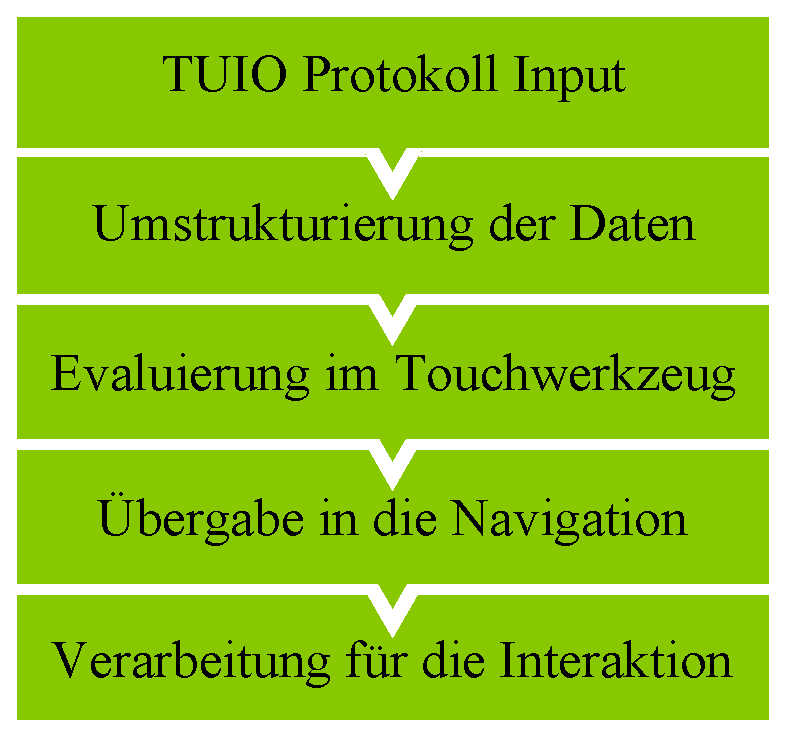
\includegraphics[width=10cm]{img/input_processing.pdf}
	\end{center}
	\caption{Verarbeitung des Touch Inputs.}
	\label{fig:input_processing}
\end{figure}

Die Verarbeitung von Touch Eingaben erfolgt in drei wesentlichen Schritten. Schritt 1 wird einmalig zu Applikationsstart ausgeführt. Hierbei wird für die Maximalanzahl an gleichzeitig erkennbaren Händen jeweils ein Touchwerkzeug angelegt. Während der MSER-Algorithmus (siehe Kapitel \ref{chp:mser}) zur Erkennung von Eingaben keine Begrenzung aufweist, sind die in der Applikation nutzbaren Inputpositionen durch die Anzahl verfügbarer \emph{Stations} im \emph{Avango Daemon} begrenzt (siehe Unterabschnitt \ref{subsec:tuio_touch_protokoll}). Touchwerkzeuge sind vom Anwender konfigurierbar und sollen die Verbindung zwischen der taktilen Eingabe und der jeweiligen Auswirkung dieses Inputs in der Applikation herstellen. Jedes Touchwerkzeug verarbeitet den Input von genau einer Hand. Des Weiteren verfügt jedes dieser Werkzeuge über verschiedene Geometrien zur Visualisierung der Eingabe. Der Input einer Hand wird als Teil des Touchwerkzeugs in einem Datencontainer gehalten, welcher bei Bedarf in Schritt 2 gefüllt wird.
\\\\
Sobald durch den in Abschnitt \ref{chp:mser} vorgestellten MSER-Algorithmus Fingerkontaktpunkte ermittelt wurden, folgt Schritt 2. An dieser Stelle werden die Daten aus dem TUIO Protokoll Transfer ausgewertet und umstrukturiert. Hierzu werden die angesprochenen Datencontainer gefüllt. Diese identifizieren jede erkannte Hand und enthalten außerdem eine Liste mit Positionen der einzelnen Finger, sowie eine errechnete Handzentrumsposition. Die Handzentrumsposition entspricht dem Mittelpunkt der um alle enthaltenen Finger gespannten Bounding Box. Durch die in Abschnitt \ref{sec:diskussion_mser} vorgestellten Komplikationen bei der Handerkennung, werden Finger nur beim ersten Aufsetzen auf die Tischplatte einer Hand zugewiesen. Bei der Eingabeverfolgung bleibt diese Zuordnung erhalten.
\\\\
Da jeder der in Schritt 2 beschriebenen Datencontainer an ein Touchwerkzeug gebunden ist, erfolgt in Schritt 3 zuletzt die Verknüpfung der Eingabe mit der jeweiligen Auswirkung in der Applikation. Hierzu verfügen Touchwerkzeuge über einen Selektionsmechanismus, welcher basierend auf den vorliegenden Eingabedaten und dem aktuellen Applikationsstatus Kontakt zu einem Applikationsmanipulator herstellt. Dieser wird über Strahlenschnitttests realisiert. Abbildung \ref{fig:input_processing} visualisiert einen Überblick über die einzelnen Schritte der Verarbeitung von Toucheingaben.

\section{Touch Navigation}
\label{sec:touch_navigation}

Touchwerkzeuge verfügen nicht über die Macht direkte Veränderungen an der Applikation vorzunehmen, ausgenommen der Darstellung ihrer eigenen geometrischen Repräsentation. Sie stellen lediglich durch die gegebenen Input Daten einen Kontakt zu Applikationsmanipulatoren her. Wir definieren diese Manipulatoren als Objekte zur funktionsspezifischen Änderung bestimmter Eigenschaften der Anwendung.
\\\\
Die Touch Navigation ist ein Applikationsmanipulator zur Umsetzung der vorgestellten Multi-Touch Techniken auf die Transformation des virtuellen Bildschirms. Die Klasse benötigt zur Bestimmung der Interaktion Eingabedaten, welche wiederum von den Touchwerkzeugen geliefert werden. Jedes dieser verfügt über einen Selektionsmechanismus, welcher genutzt wird um Kontakt zu Applikationsmanipulatoren wie auch der Touch Navigation aufzubauen. Diese verfügt über eine durchsichtige Geometrie, welche an den physikalischen Bildschirm angehängt wird. Sie referenziert dadurch den für die Eingabe nutzbaren Bereich. Beim Aufsetzen einer Hand wird das zugewiesene Touchwerkzeug aktiviert und führt zwei Strahlenschnittteste aus. Der erste bestimmt den Auftreffpunkt auf der sichtbaren Szenengeometrie. Durch den zweiten Schnitt wird funktionale Geometrie getestet. Dies schließt die Fläche, welche durch die Touch Navigation definiert wurde, sowie etwaige Menüelemente ein. Neben einer Auftreffposition bietet der Schnitt mit funktionaler Geometrie auch die Referenz auf eine bestimmte Klasse. Auf diese Weise kann das Touchwerkzeug durch erfolgreichen Schnitttest der durchsichtigen Fläche auf dem Bildschirm Zugriff auf die Touch Navigation erhalten.
\\\\
Jeder Applikationsmanipulator ist mit den Funktionen \emph{addContact} und \emph{removeContact} ausgestattet. Nachdem das Touchwerkzeug eine funktionale Geometrie getroffen hat, wird auf der Referenzierten Klasse \emph{addContact} aufgerufen. Diese Funktion wird mit den Eingabedaten des Touchwerkzeugs, einer eindeutigen Identifikationsnummer (ID) für die Bindung, sowie dem Geometrieschnitt des Szeneninhalts parametrisiert. Wird der Kontakt von der Touch Navigation entgegengenommen, speichert das Werkzeug die Bindung und leitet etwaige Veränderungen des eigenen Inputs über \emph{addContact} an den Manipulator weiter. Andernfalls gilt der gegebene Input als blockiert und das Touchwerkzeug hat keine Auswirkung auf die Navigationsinteraktion. Um an den Manipulator gebunden werden muss sich ein gebundener Kontakt lösen und das Touchwerkzeug erneut anmelden. Letzteres ist nach Lösen eines gebundenen Kontakts durch erneutes Aufsetzen der Hand möglich. Da die Touchwerkzeuge keinem Nutzer zugeordnet werden können, wird auf diese Weise die gleichzeitige Interaktion mehrerer Nutzer eingeschränkt. Verliert ein Werkzeug durch Anheben der jeweiligen Hand die Eingabe, so wird der Kontakt durch \emph{removeContact} parametrisiert durch seine zugehörigen ID, von der Navigation abgemeldet.
\\\\
Die Touch Navigation verwaltet eine Liste von Touch-Kontakten welche, durch die in Abschnitt \ref{sec:evaluierung_der_bildschirmkontakte} beschriebenen Zusammenhänge, auf eine Länge von zwei Elementen begrenzt ist. Erhält der Manipulator eine Bindungsanfrage über \emph{addContact}, urteilt er anhand der Elemente in dieser Liste wie mit der Anfrage umzugehen ist. Existiert bereits ein Kontakt mit gleicher ID, wird eine Aktualisierung dieses basierend auf den gelieferten Daten durchgeführt. Falls nicht und ist die Maximalanzahl der gleichzeitig verwertbaren Touch-Kontakte nicht erreicht, wird der Liste ein weiteres Element beigefügt. Die Anfrage wird in beiden Fällen als erfolgreich beantwortet. Ist die Kapazität der Listenbegrenzung erreicht und entspricht die ID nicht der eines in der Liste enthaltenen Elements, wird der Kontakt verworfen. Folglich wird die Anfrage als nicht erfolgreich beantwortet.


\section{Repräsentation im Szenegraph}
\label{sec:rep_im_szenegraph}

Im Gegensatz zu anderen physischen Werkzeugen ist der Multi-Touch Bildschirmtisch kein nutzerspezifisches Eingabegerät. Präzise ausgedrückt handelt es sich vielmehr um ein Mehrbenutzer Display mit Interaktionsschnittstelle. Demnach ist der Touch-Tisch gleichzeitig Darstellungs- sowie Eingabemedium, was für die Modellierung im Szenegraph berücksichtigt werden muss. 
\\\\
Die Konstruktion der Repräsentation des Tisches als virtuelles Display wird durch das verwendete Applikationsframework vorgenommen. In Abschnitt \ref{sec:multitouch_input_pipeline} wurden Touchwerkzeuge als Teil der Multi-Touch Input Pipeline vorgestellt. Ihre Geometrie visualisiert die  von ihnen genutzten Inputdaten auf dem Bildschirm, sowie die Verbindungsgerade der von ihnen ermittelten Schnittposition mit der Szenengeometrie. Touchwerkzeuge können bislang nicht eindeutig einem bestimmten Nutzer zugeordnet werden, jedoch sind ihre Visualisierungen immer von der Transformation des Bildschirms abhängig. Des Weiteren sind die durch sie angestoßenen Interaktionsanfragen logischer Teil der Eingabe durch den Multi-Touch Tisch. Aus diesem Grund wird die Geometrie der Touchwerkzeuge dem Bildschirmknoten angehängt.
\\\\
Auf eine Eltern-Kind Beziehung zwischen Hand und den Fingern wurde absichtlich verzichtet. Da die Fingerpositionen bei der Eingabe im Bildraum ausgedrückt sind, müssten sie hierfür in den Objektraum des Handknotens transformiert werden. Durch ständige Neupositionierung der Finger und folglich auch der Hand, würde diese Umwandlung die Performanz beeinträchtigen.


\section{Diskussion}
\label{sec:diskussion_applikationsstruktur}

Da die meiste Interaktion ausgehend von einzelnen Händen, anstatt von Fingern, abgeleitet wird erscheint die Verwendung des Touchwerkzeugs als Datenstruktur naheliegend. Um die Eingabe der Werkzeuge zu steuern wird eine Umstrukturierung der Daten in der Applikation vorgenommen. Diese kostet Zeit und wirkt sich daher negativ auf die Performanz des Systems aus. Mit der einmaligen Handzuordnung wird die Toucherkennung merklich stabilisiert.
\\\\
Das Konzept der Applikationsmanipulatoren macht die vorgestellte Struktur leicht erweiterbar. Bei der Programmierung können neue Manipulatoren eingeführt werden, welche durch den Selektionsmechanismus der Touchwerkzeuge bedient werden. Hierbei muss das Werkzeug die Klasse nicht kennen, solange sie die \emph{addContact} und \emph{removeContact} Funktionalität unterstützt. Hierbei scheint jedoch die Wahl des Schnitttests unsichtbarer Geometrie als Selektionsmechanismus verbesserungswürdig.
